


\section{Measuring conflict}
\label{sec:chapter1-measurement}

As we have seen, there are a number of points at which
we might expect conflict to occur during high-level reasoning.
If we are to study this conflict, however,
the data we collect must reflect it.
This is not always straightforward.
While recent technological advances have made it possible
to know whether of not neurons in a given part of the brain,
or under some circumstance even specific neurons, are firing,
we remain some distance from being able to
describe complex cognitive phenomena
in terms of these underlying, observable, biological processes.
Instead, experimental cognitive psychologists make us of an approach
inherited from the Behaviourist tradition:
we present our participants
with experimentally controlled stimuli,
and we record what occurs as a result,
either in terms of overt responses,
or more subtle measures that shine a light on underlying processes.

In this section, I review methods previously used in the study 
of both reasoning, and of conflict more broadly.
These range from analyses of participants' discrete responses,
to response latencies, to subtler paradigms that reveal
something of underlying processes, such as fMRI and eye tracking. 
I also introduce the mouse tracking paradigm,
which forms the basis of the experiments reported
later in this thesis.


\subsection{Responses}
\label{subsec:chapter1-measurement-responses}

The basic experimental paradigm used by cognitive psychologists
has changed little over the last 50 years:
participants are presented with stimuli,
ranging from a simple perceptual probes
to complex verbal problems,
and asked to provide a discrete response,
either verbally, numerically, or by pressing a button.
Thus, most %% much? 
psychological research rests on
the analysis of only these single responses,
collected after the process of interest has terminated.
More complex designs,
incorporating confidence ratings or list sorting,
for instance, add some nuance to the analysis,
but remain focused on the end product of the cognitive process.
Collecting only these responses in a single condition,
or in simple experiments,
it is not possible to detect conflict directly,
but such data can reveal what factors drive decisions.
For instance, as discussed above, \citet{Gelman1986} 
presented children with a forced choice,
asking them to generalise properties either
between entities that belong to the same category,
but look different,
or between entities that are visually similar,
but belong to different categories.
By demonstrating that children overwhelmingly choose
to generalise based on category membership,
they concluded that category knowledge
drives inductive inference in children.


True experiments, in which the factor of interest
is manipulated between conditions,
provide a better test of what influences final choices.
\citet{Evans1983} asked participants to decide
if presented syllogisms were valid or invalid,
and manipulated if the arguments' conclusions
were believable, or unbelievable.
Finding that participants were more likely to class arguments
with believable conclusions as valid,
both for valid and invalid items,
they concluded that belief and logic conflicted on the task.
Response data can also be combined with a range of
information about individual differences between participants
in correlational analyses.
\citet{Stanovich1999,Stanovich2000,Stanovich2008}, for instance,
showed that for a number of tasks in which
intuition and logic are thought to conflict,
the number of logically correct responses a participant produces
can be variously predicted by their IQ,
or by personality measures.

However, terminal responses remain only an indirect indicator of conflict:
it is difficult, for instance, to differentiate between
a manipulation that elicits conflict between multiple processes,
and one that merely changes the kind of processing participants engage in.
There are many measures we can collect
that reveal more about underlying processes,
but the most popular of these are response latencies.


\subsection{Response Latency}
\label{subsec:chapter1-measurement-latency}


With the use of personal computers to collect data,
it is easier than ever to record
not only the responses participants give,
but how quickly they give them --- their \emph{response latencies}.
This \emph{chronometric} approach has a long history,
particularly in the individual differences, or \emph{psychometrics} tradition 
\citep[see][for reviews]{Posner1978, Meyer1988}.
Response latencies have obvious advantages over simple responses
in the detection of conflict during cognition.
Although conflict may not affect the responses participants give,
slower responses are indicative of greater difficulty
in generating these responses,
often as a result of the need to resolve or inhibit conflict.
In the Stroop task \citep{Stroop1935},
participants are asked to verbally identify the colour in which words are printed.
Doing so may involve conflict when
the words themselves are colour names
and the printed word and ink colour differ:
participants must inhibit an automatic tendency
to read the colour name aloud
in order to properly perform the task.
In non-clinical populations,
error rates on this task are typically very low,
but conflict, and individual differences in the ability to resolve this conflict,
can be inferred by comparing response latencies
for congruent and incongruent colour names.
The same principle has been applied to forced choice tasks,
including the Eriksen flanker task \citep{Eriksen1974},
in which participants are required to respond
on the basis of a centrally located probe,
ignoring flanking stimuli on either side
which may be congruent, incongruent, or neutral.
Similarly, in the Simon task \citep{Simon1963},
stimuli can be presented centrally on a display,
or lateralised to either side.
Responses with the right hand are slower
to stimuli presented in the left visual field,
and vice versa.

One issue that arises in the analysis of response latencies
is the relationship between response time and choices.
On tasks in which more than one response is possible,
and there is variance in the choices participants do make,
there is often a \emph{speed-accuracy trade-off},
with participants striking a balance between
maximising speed, and thus sacrificing accuracy,
or vice versa \citep{Garrett1922}.
A popular solution to this problem has been to
fit models of the underlying decision process
that account for both the participants' choices
and their corresponding response times.
\emph{Sequential sampling models}
\citep{Ratcliff1978,Ratcliff2008a,Busemeyer1993,Hawkins2015}
are commonly used for this purpose.
These model both participants' responses
and their response latencies
as a process of accumulating evidence over time.
However, despite the strengths of recent modelling-based approaches
in inferring underlying processes from responses latencies,
the data upon which these models are based
remain after-the-fact products of the processes we are interested in.
Greater sensitivity still comes from a family of methods
known as \emph{``process tracing''} that seek to monitor
these cognitive processes as they happen.






\subsection{Process Tracing}
\label{subsec:chapter1-measurement-process-tracing}

Process tracing paradigms are those where
cognitive processes, or their correlates, are recorded as they unfold.
These paradigms range from asking participants to think aloud,
to measurement of neural and biological states, including fMRI and EEG,
to recording of eye gaze in order to infer attention during cognition,
and to mouse tracking, the method which will form the core of this thesis.

Protocol analysis \citep{Ranyard2010,Ericsson1980},
where participants are asked to explicitly ``think aloud'' while performing a task,
is perhaps the most straightforward such method.
Often, this involves experimenters specifying, a priori,
the possible strategies participants may use,
or the information they may make use of,
and identifying from participants' verbal reports
which of these were actually used.
In reasoning research,
\citet{Evans1983} make use of this approach
in conjunction with experimental data,
showing that when asked to evaluate the logical validity of syllogisms,
participants were influenced by whether or not
the conclusion of the syllogism was believable,
and that participants explicitly reported taking belivability into account
when completing the task.
Of course, as noted by \citet{Nisbett1977},
not all cognitive processes are available to introspection.
Therefore, this paradigm works best as a measure of 
the steps participants are explicitly aware of taking,
or the information they were explicitly aware of using, during a task.
For instance, \citet{DeNeys2008} showed that while
implicit measures showed that participants were sensitive to
conflicts between their biased inferences and statistical information,
participants rarely made reference to this statistical information,
suggesting that this conflict detection was achieved implicitly.

Other methods go beyond the limitations
of relying on participants' self reported mental states.
There has been a huge body of research, across many fields,
on the neural and biological correlates of cognition and their measurement,
which I can only briefly list here.
Functional Magnetic Resonance Imaging \citep[fMRI;][]{Huettel2004}
is perhaps the best-known of these techniques,
and reveals the firing rate of populations of neurons
by monitoring the oxygen content of inflowing blood.
This provides excellent spatial resolution,
but at a substantial temporal delay.
In contrast, electroencephalography \citep[EEG;][]{Niedermeyer2005}
and less commonly magnetoencephalography \citep[MEG;][]{Hamalainen1993}
record the weak electrical and magnetic fields generated by active neurons,
allowing for extreme temporal accuracy in inferring neural activation,
but with limited spatial acuity.

The usefulness of these methods in studying cognitive tasks
relies on the assumption that cognitive processes can be
directly mapped onto the activation of specific neural regions,
or to characteristic signals time-locked with the onset of the relevant stimuli 
(Event Related Potentials).
Fortunately, although this assumption
has been questioned in a number of domains \citep[see][]{Coltheart2013},
there appear to be clear neuroanatomical mappings
in the case of conflict in cognition.
Specially, the detection of conflict between processes
is known to be strongly correlated with activation of the ACC \citep{Botvinick2004},
while the processes of inhibiting conflicting processes
engages the prefrontal cortex \citep{Aron2004,Miller2001}.
Thus, the logic of studying conflict using these measures is clear:
a manipulation can be claimed to induce conflict
if it leads to greater activation of the ACC,
and participants who show greater PFC activation
are engaged in the inhibition of a conflicting process
\citep[see, i.e.][]{DeNeys2008}.

Other biological measures exist that
do not directly reflect neural activity,
including galvanic skin conductance \citep{DeNeys2010, Figner2010},
and pupil dilation \citep{Fiedler2012, Kahneman1966, Wang2011}.
All of these measures reflect arousal of the autonomic nervous system,
which in turn is influenced by \emph{cognitive load}
\citep{Kahneman1966}.
However, like the neural measures reviewed above,
the processes measured in these paradigms
are not the cognitive phenomena in which we are primarily interested,
but epiphenomenal by-products,
or at best physical correlates of the mental processes.

An alternative to analysing these by-products
is to look to a process that we know to precede cognition: attention.
Although some work \citep[i.e.][]{Evans1996a} has asked participants
to explicitly indicate the locus of their attention,
the most commonly used measure of attentional focus
is the eye tracking paradigm.
Eye tracking has a long history in psychology
(\citealp{Ball2014, Mele2012, Huey1908, Yarbus1967};
see \citealp{Duchowski2007} for a review)
and in its modern form typically relies on
using a camera to record the reflection of infrared light
off different parts of the eye.
Popular uses of the method include
measuring attention as part of complex behaviours
such as social interaction \citep[i.e.][]{Hanley2014},
decision making \citep{Krajbich2011}
and reasoning \citep{Ball2014},
as well as in scenarios in which the low-level processes
driving gaze fixation themselves are of interest,
such as during reading \citep{Rayner1998}
and visual search \citep{Treisman1980}.
The strengths of the eye tracking paradigm are clear.
It provides an unobtrusive measure of participants' attention,
with impressive spatial and temporal resolution,
across almost any cognitive task.

As a paradigm, eye tracking is also extremely flexible,
and eye tracking data can be analysed in a number of ways.
Perhaps reflecting the popularity of eye tracking in psycholinguistics,
many experiments use eye tracking data
to infer how long participants spend reading particular passages of text,
reflecting the time spent processing particular information, or its unexpectedness.
It is additionally possible to differentiate between
effects which manifest quickly
(which affect participants' first pass over the text in question)
and those which occur later (which affect processing of subsequent text,
or regressions back into the text in question).
\citet{Haigh2014}, for instance,
presented participants with vignettes where
a particular inference could be drawn early in the text,
and showed that participants slowed down on their first pass through
sentences which were inconsistent with that inference,
indicating that the inference was made quickly and automatically while reading.
Alternatively, participants' gaze can reflect
the extent to which they are considering certain options.
\citet{Ball2003} used eye tracking in this way,
analysing participants' \emph{inspection times} for each card
on the \citet{Wason1968} selection task.
They found that participants were more likely
to initially inspect cards cued by Type 2 processes
(those mentioned by name in the instructions),
and subsequently more likely to select cards if they inspected them initially.
Reanalysis of this data by \citet{Evans2010}
showed that Type 2 processes also played a role,
as participants were more likely to select a card
after initially inspecting it when doing so was the logically correct thing to do.

Eye tracking is also a useful tool when studying conflict.
In the popular Visual World paradigm
\citep{Huettig2011,Allopenna1998,Tanenhaus1995},
for instance, participants are instructed over headphones
to interact with a display in front of them, or on a computer screen.
On some trials, there was syntactic ambiguity in these instructions ---
for example, they begin ``place the apple on the towel ...''
when the display includes an apple, a towel, and a second apple on a second towel;
it is not clear if the task is to place the first apple onto the towel,
or move the apple that is already on the towel elsewhere.
In these cases, participants look to both possible referent,
before later information (e.g. ``... into the box'') disambiguates the referents.
In a similar vein, \citet{McMurray2008} asked participants to 
categorise phonemes that were intermediate between
simple consonants such as ``[d]'' vs. ``[g]''.
Although participants typically report
\emph{categorical perception} of one or other consonant,
they looked more often at the alternative response option
as the stimuli became more ambiguous, indicating conflict. 
Intriguingly, \citet{Richardson2000} demonstrated
that eye tracking can also reveal retrieval from memory,
as participants look at regions of the screen
where information was presented when recalling that information.
Finally, while most analyses of eye tracking experiments
reduce the data down to single summary measures  ---
for instance, time spent looking at each response option ---
it is also possible to analyse the data as a continuous time series.
Recently, several psycholinguistics researchers have explored
the use of multilevel regression techniques
to make sense of eye tracking data in such a way
\citep[e.g.][]{Barr2008,Mirman2014a,Mirman2008}.
I will return to these methods in Chapter 2.

One notable shortcoming of the eye-tracking paradigm
in studying high-level cognition, however,
is that the connection between attention
and the underlying processes of interest cannot always be taken for granted.
If we find that participants look more to one option than another,
for instance, it is difficult to tell if
they look to this option because they wish to choose it,
they wish to choose this option because they have looked at it,
or some interaction of the two \citep[see][]{Krajbich2011}.
Furthermore, there is always a possibility, difficult to eliminate,
that participants look to something not because they wish to choose it,
but because they wish to rule it out.
Beyond this, participants can obviously only look at one thing at a time,
and eye movements typically consist of 
a series of \emph{saccades}: rapid, discrete movements
between one fixation point and another, in a straight line.
Generally, researchers will circumvent this issue
by aggregating participants' fixations:
if they look to option A half the time, and  option B the remainder,
then they are judged to be equally drawn towards both option.
The issue remains, however, that researchers are required to
construct often complex theoretical models
as a bridge between hypothesised psychological processes
and observed eye tracking data.

\subsection{Mouse Tracking}
\label{subsec:chapter1-measurement-mousetracking}

The mouse tracking paradigm,
introduced by \citet{Spivey2005},
goes some way towards overcoming
some of these problems inherent to eye tracking.
In this, participants' mouse cursor movements are recorded
as they complete forced-choice tasks,
and analysed to infer the extent to which
participants are drawn towards each response option
over the course of a trial.
Therefore, this paradigm appears to provide
a window into the temporal dynamics of
participants' developing beliefs over the course of a trial.
It is this paradigm that I will use throughout this thesis,
and so I will provide a general introduction to it
in the current chapter,
before discussing technical aspects of the paradigm in detail in Chapter 2.

In \citegap{Spivey2005}{'s} original experiment,
participants saw a computer display
containing images of  common objects in the top corners (see Figure~\ref{fig:spivey}).
Over headphones, they heard the name of one or other object,
and were required to click on the relevant image.
For some trials, the two objects were \emph{phonological competitors},
meaning that their names shared onset phonemes, such as ``\underline{\emph{pic}}ture'' and ``\underline{\emph{pic}}kle'',
while for others they did not.
On these conflict trials, participants' mouse cursor trajectories
displayed what has been termed \emph{continuous attraction},
moving initially towards a point between the two images,
before eventually homing in on one or other option.
A classical view of language comprehension \citep{Fodor1983}
holds that speech recognition is handled by a \emph{perceptual module},
which processes its input, and then passes on its output.
However, these results indicate that
the speech recognition instead feeds continuously into other processes,
including those executed by the motor system, in real time.
\citet{Spivey2005} argue that these data
support a \emph{continuous dynamic} model of language comprehension,
where spoken words initially partially activate
representations of multiple words consistent with the stimuli,
before this competition is resolved in favour of a single candidate word \citep[see also][]{Spivey2007}.
While the issue of language comprehension will not be the focus of this thesis,
this first application of the mouse tracking paradigm demonstrates some of its value.
Based on their mouse data, \citet{Spivey2005} were able
to demonstrate two things.
First, they showed that conflict takes place during their task.
Second, they showed that this conflict is continuous in nature
(participants were simultaneously drawn towards both response options),
rather than discrete 
(initially be drawn towards one response,
before changing their mind mid-trial).

\begin{figure}[ht]
  \centering
  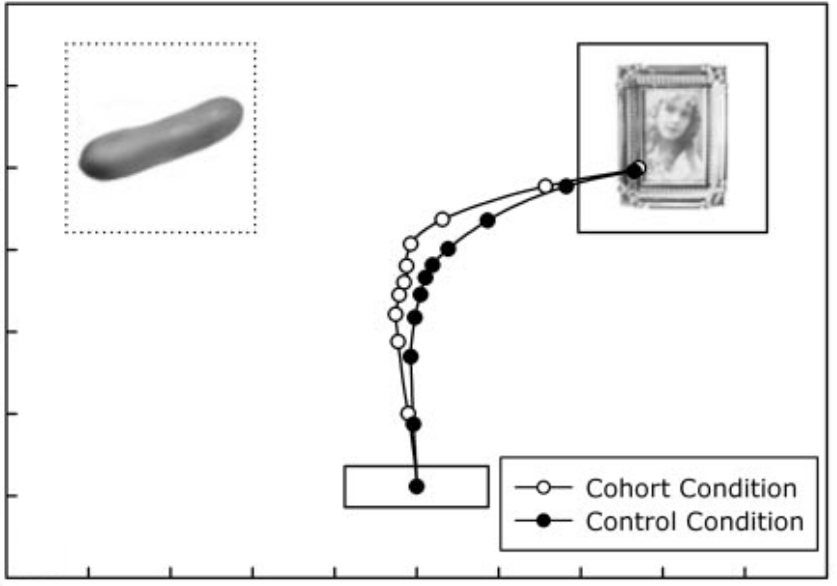
\includegraphics[width=.7\textwidth]{imgs/spivey.png}
  \caption[The mouse tracking paradigm used by \citet{Spivey2005}]{
    \citegap{Spivey2005}{'s} mouse tracking paradigm.
    Participants were told aurally to click on the ``picture''.
    Their mouse cursor trajectories showed a greater, graded attraction
    towards the alternative icon in the cohort (conflict) condition,
    where it showed a phonological competitor (PICKLE), than in the control condition,
    where it did not.
    \label{fig:spivey}
  }
\end{figure}


Therefore, mouse tracking can reveal more than simply the presence of conflict.
For instance, \citegap{Spivey2005}{'s} original mouse tracking experiment,
and many since, have reported continuous attraction effects ---
participants were partially and simultaneously drawn towards both
response options at the same time, resulting in a curved trajectory.
Other studies, however,
\citep[e.g.][]{Dale2011,Freeman2014a,Tomlinson2013,Barca2015,Resulaj2009}
have revealed more discrete effects,
as participants move directly towards one or other option,
but sometimes change direction mid-flight.
In this way, mouse tracking can show us something
of the qualitative nature of conflict during a task.
In Appendix~\ref{appendix:mouse-studies},
I have compiled a table showing some of the mouse tracking studies
that have found graded, continuous attraction effects,
and some of those that have shown discrete reversals, or changes of mind.
I return to the issue of reversals in cursor trajectories
from a practical point of view in Chapter 2,
and again from a theoretical point of view in Chapter 7.

Mouse tracking may also reveal something of
\emph{when} conflict occurs,
or at what point in time various factors influence participants' cursor movements.
For example, \citet{Freeman2011c} asked participants to categorise faces
according to either their gender, or their age (young or old),
and manipulated both the pigmentation and the shape of faces to be
either category-typical or category-atypical.
They found that face pigmentation affected cursor trajectories
for gender categorisation 50 ms before face shape did,
and that the effect of pigmentation manifested
100 ms earlier for gender categorisation than for age categorisation.




% Other mouse tracking
At this point, it is worth highlighting that this procedure
is not the only known ``mouse tracking'' paradigm.
Analysis of computer mouse cursor locations
have been used for some time as a measure of 
participants' information search, or attention,
during cognitive tasks.
Information search experiments are typically implemented in two ways,
using either the ``flashlight'' procedure 
\citep{Schulte-Mecklenbeck2011, Yamauchi2007},
in which regions of the screen are blurred or dark,
and the mouse must be pointed directly at them in order to see the relevant stimuli,
or the MouseLab procedure \citep{Willemsen2011},
in which information is presented in tables with occluded cells,
that participants must click or hover over to temporarily reveal.
In a related paradigm, participants' patterns of attention
can be monitored by explicitly asking them
to point the cursor at the focus of their attention
\citep{Evans1996, Evans2010, Stupple2008}.
This method likely provides a low-cost proxy
for more difficult eye tracking methods.

Another field of research making use of mouse cursor data
is work by those interested in human computer interaction.
As the mouse cursor is the natural means
of interacting with computer interfaces, such as web pages,
analysing mouse movements provides a naturalistic measure of 
the effects of manipulating their layout and content
\citep[e.g.][]{Huang2011, Cox2006}.
Work combining mouse and eye tracking \citep{Chen2001, Rodden2008}
has shown that while mouse movements correlate with gaze,
they also are used in more task-specific ways, 
such as hovering near potential selections as a marker
while gaze is used to explore other less likely candidates.
I will return to these alternative notions of mouse tracking in Chapter 6,
where a novel mouse tracking paradigm is introduced.
However, for the first three experimental chapters of this thesis,
the paradigm used will be essentially that used by \citet{Spivey2005}.

